%-------------------------
% Resume in Latex
% Author : Javier Tarazona
%------------------------

\documentclass[letterpaper,10pt]{article}
\DeclareUnicodeCharacter{00A0}{~}
\DeclareUnicodeCharacter{2013}{\textendash}
\DeclareUnicodeCharacter{2014}{\textemdash}
\DeclareUnicodeCharacter{201C}{``}
\DeclareUnicodeCharacter{201D}{''}
\DeclareUnicodeCharacter{2022}{\textbullet}
\DeclareUnicodeCharacter{25E6}{\textopenbullet}
% \setlist[itemize]{label=\textbullet, labelsep=0.5em, leftmargin=*} % Moved after \begin{document}
\usepackage[T1]{fontenc}      % Codificación de salida (acentos y símbolos)
\usepackage[empty]{fullpage}
\usepackage[export]{adjustbox}
\usepackage[pdftex]{hyperref}
\usepackage[usenames,dvipsnames]{color}
\usepackage[utf8]{inputenc}   % Lee texto en UTF-8
\usepackage{array}
\usepackage{comment}
\usepackage{enumitem}
\usepackage{enumitem}         % Control de listas (si no lo tienes ya)
\usepackage{fancyhdr}
\usepackage{graphicx}
\usepackage{latexsym}
\usepackage{lmodern}
\usepackage{marvosym}
\usepackage{tabularx}
\usepackage{titlesec}
\usepackage{verbatim}
\usepackage{xcolor}


\usepackage{latexsym}
\usepackage[empty]{fullpage}
\usepackage{titlesec}
\usepackage{marvosym}
\usepackage[usenames,dvipsnames]{color}
\usepackage{verbatim}
\usepackage{enumitem}
\usepackage[pdftex]{hyperref}
\usepackage{fancyhdr}
\usepackage{tabularx}
\usepackage{graphicx}
\usepackage{array}
\usepackage[export]{adjustbox}
\usepackage{xcolor}
\usepackage{comment}

\begin{comment}  
\end{comment}
% --- Codificación y fuentes seguras ---
\usepackage[utf8]{inputenc}   % Lee texto en UTF-8
\usepackage[T1]{fontenc}      % Codificación de salida (acentos y símbolos)
\usepackage{enumitem}         % Control de listas (si no lo tienes ya)

% --- Viñetas limpias y seguras ---
\setlist[itemize]{label=\textbullet, labelsep=0.5em, leftmargin=*}
%\end{comment}

\pagestyle{empty}

% Adjust margins
\addtolength{\oddsidemargin}{-0.45in}
\addtolength{\evensidemargin}{-0.45in}
\addtolength{\textwidth}{1.15in}
\addtolength{\topmargin}{-.62in}
\addtolength{\textheight}{1.20in}

\urlstyle{same}

\raggedbottom
\raggedright
\setlength{\tabcolsep}{0in}
\renewcommand{\arraystretch}{0.98}

%\definecolor{mydarkgreen}{RGB}{0, 140, 123}
\definecolor{mydarkgreen}{RGB}{0, 0, 0}

% Sections formatting
\titleformat{\section}{
  \vspace{-5pt}\scshape\raggedright\large
}{}{0em}{}[\color{mydarkgreen}\titlerule \vspace{-6pt}]

%-------------------------
% Custom commands
\newcommand{\resumeItemCompact}[2]{\item\small{\textbf{#1}: #2}\vspace{-2pt}}
\newcommand{\resumeItemListStartCompact}{\begin{itemize}[leftmargin=*,itemsep=0pt,parsep=0pt,topsep=0pt,partopsep=0pt,nolistsep]}
\newcommand{\resumeItemListEndCompact}{\end{itemize}\vspace{-4pt}}

\newcommand{\resumeItem}[2]{
  \item\small{
    \textbf{#1}{: #2 \vspace{-2pt}}
  }
}

\newcommand{\resumeSubheading}[4]{
  \vspace{-1pt}\item
    \begin{tabular*}{0.97\textwidth}{l@{\extracolsep{\fill}}r}
      	\textbf{#1} & \textbf{\textcolor{mydarkgreen}{#2}} \\
      	\textit{\footnotesize#3} & \textit{\footnotesize \textcolor{mydarkgreen}{#4}} \\
    \end{tabular*}\vspace{-4pt}
}

\newcommand{\resumeSubItem}[2]{\resumeItem{#1}{#2}\vspace{-4pt}}

\renewcommand{\labelitemii}{$\circ$}

\newcommand{\resumeSubHeadingListStart}{\begin{itemize}[leftmargin=*]}
\newcommand{\resumeSubHeadingListEnd}{\end{itemize}}
\newcommand{\resumeItemListStart}{\begin{itemize}[itemsep=0pt,parsep=0pt,topsep=0pt,partopsep=0pt]}
\newcommand{\resumeItemListEnd}{\end{itemize}\vspace{-5pt}}

% Indented paragraph helper: \indentbox[ancho]{contenido}
% Uso: \indentbox{Texto...}  o  \indentbox[1.5em]{Texto...}
\newcommand{\indentbox}[2][1em]{\hspace*{#1}\parbox{\dimexpr\linewidth-#1\relax}{#2}}

\newlength{\headerPhotoSpace}
\setlength{\headerPhotoSpace}{0pt}
\newcommand{\showHeaderPhoto}{%
  \setlength{\headerPhotoSpace}{0.13\textwidth}%
  \makebox[0pt][l]{\adjustbox{valign=c}{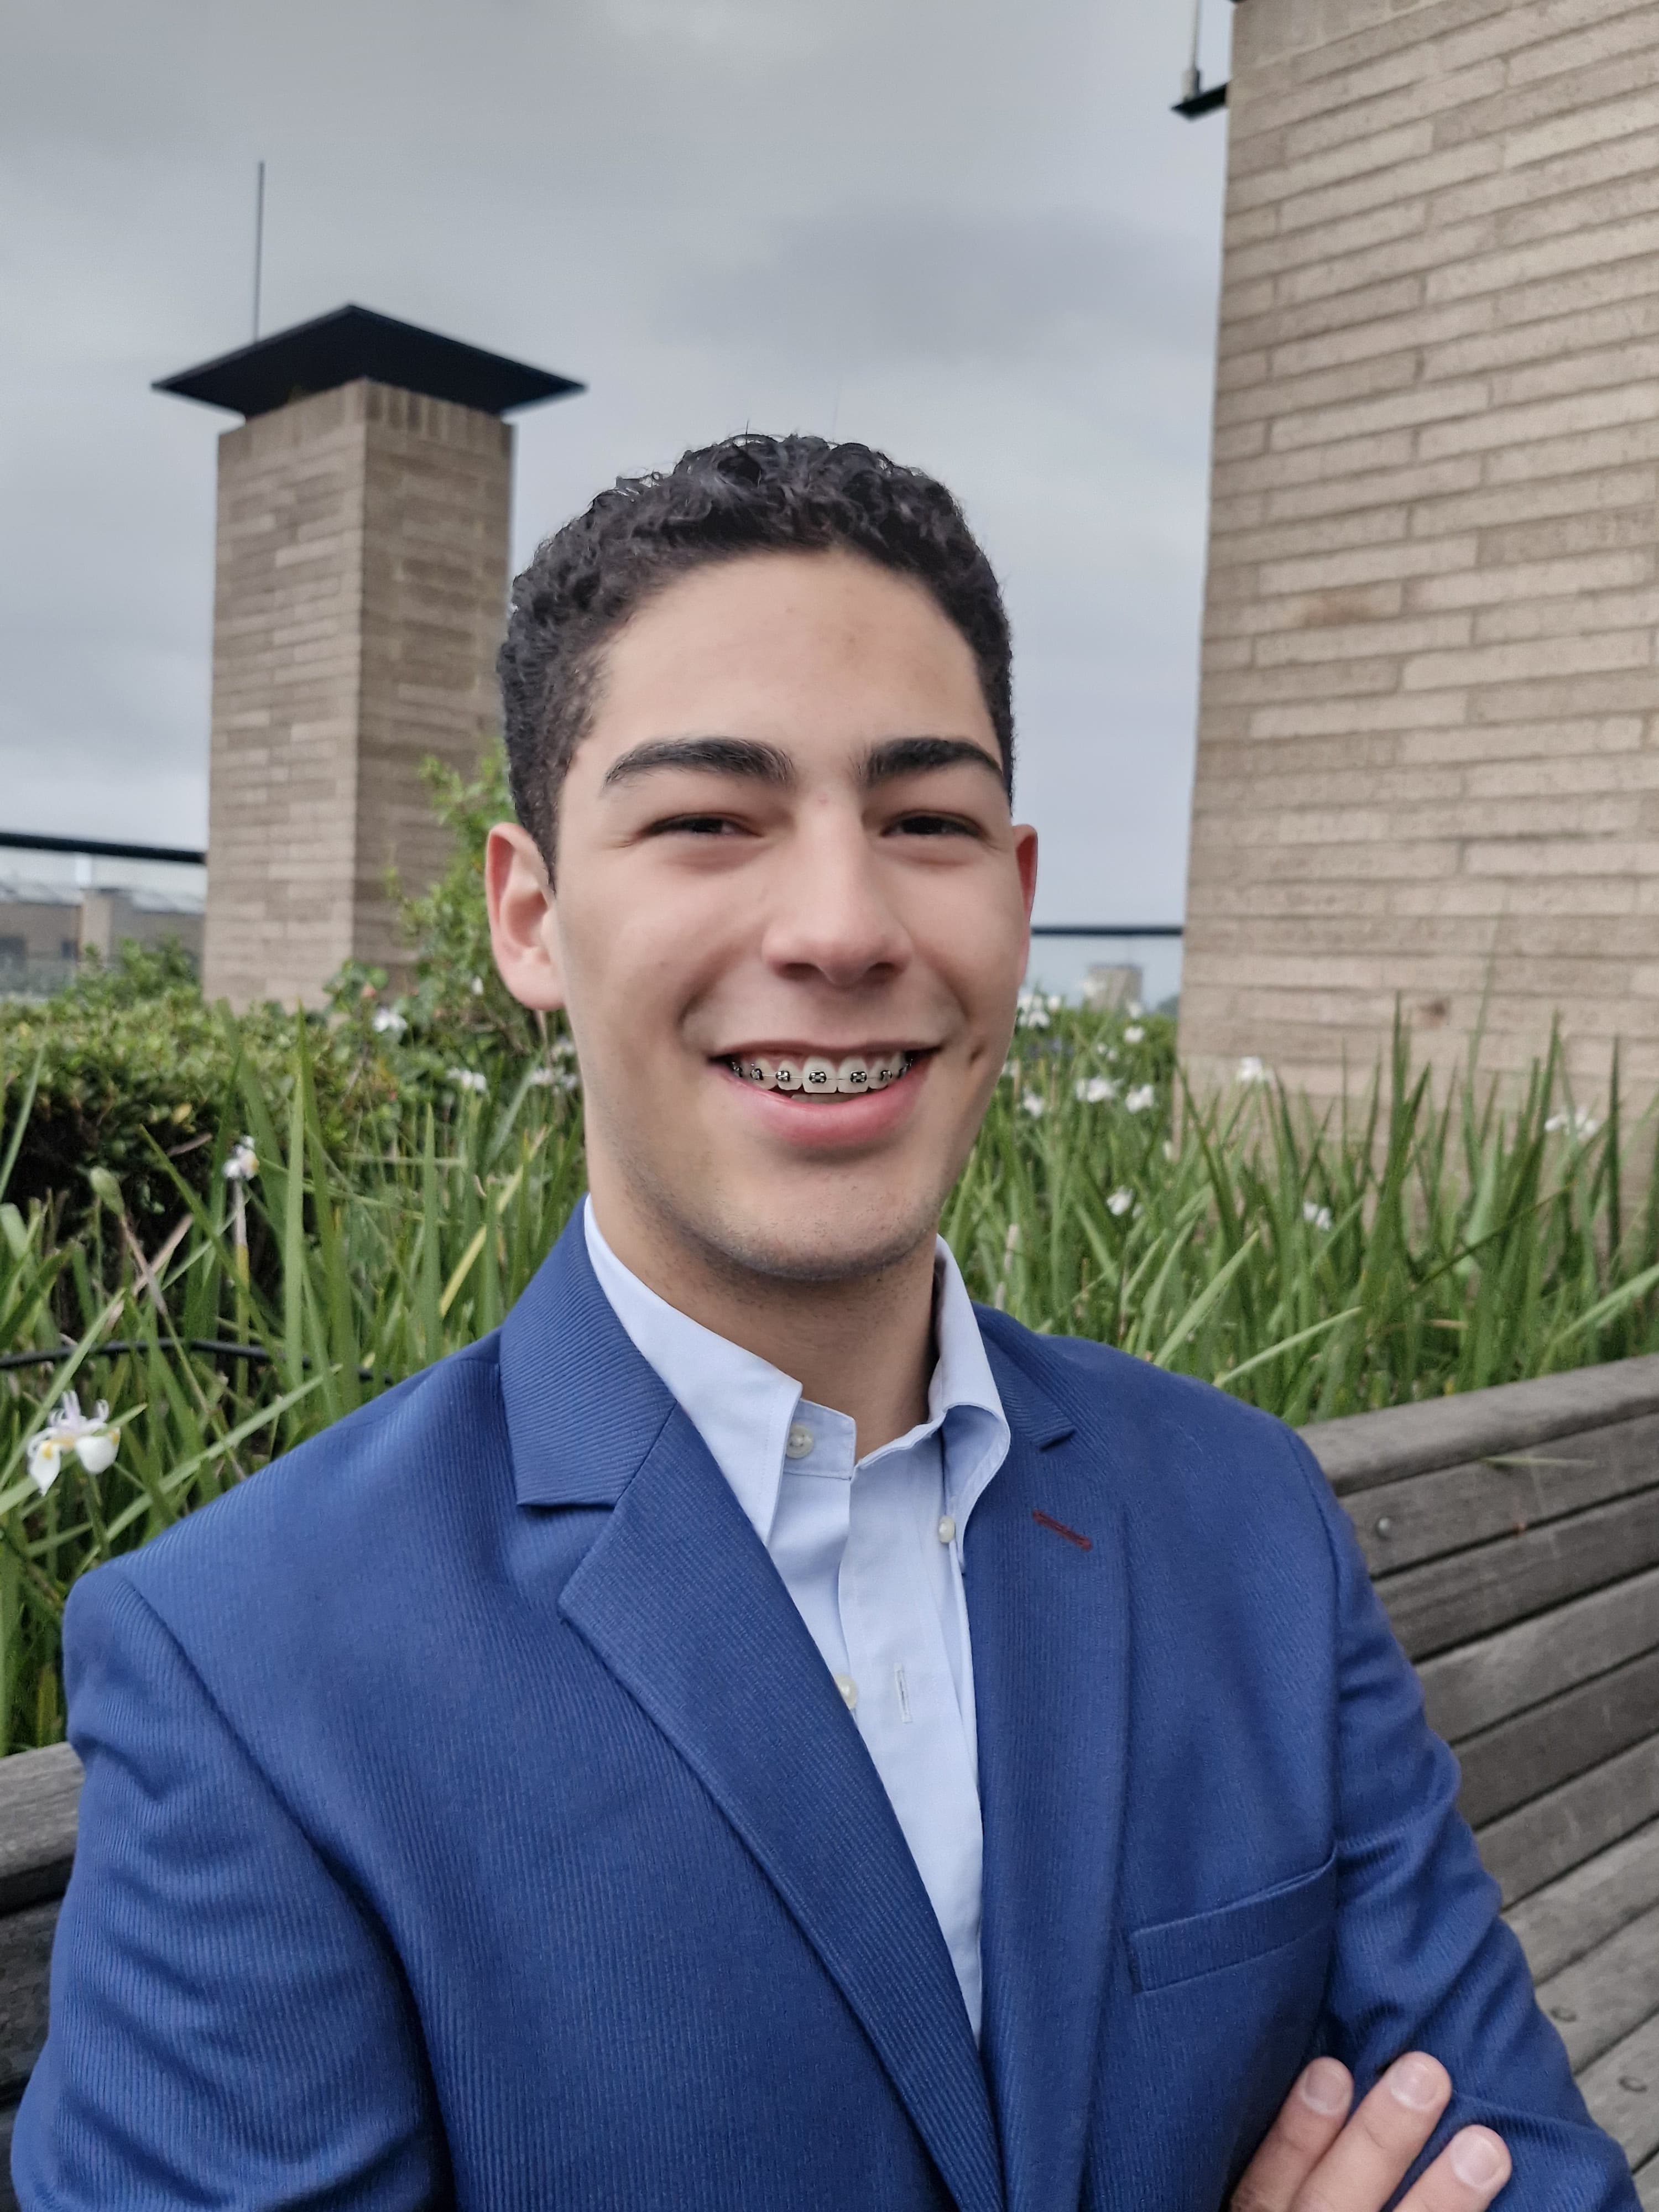
\includegraphics[scale=0.015]{Digital_photo.jpg}}}%
}


%-------------------------------------------
%%%%%%  CV STARTS HERE  %%%%%%%%%%%%%%%%%%%%%%%%%%%%


\begin{document}

\begin{comment}
\AddToHookNext{shipout/foreground}{%
  \put(\dimexpr\paperwidth-0.35cm\relax,-\dimexpr\paperheight-0.35cm\relax){%
    \makebox(0,0)[rb]{%
      \begin{minipage}{2.15cm}
        \centering
        {\setlength{\fboxsep}{1pt}\colorbox{white}{%
          \parbox{1.9cm}{\centering\scriptsize\bfseries Scannez le QR \\[-1pt]pour la version numérique}}}\\[1pt]
        
\includegraphics[width=1.6cm]{qr_CV.png}%
      \end{minipage}%
    }%
  }%
}
\end{comment}

% --- Viñetas limpias y seguras ---
\setlist[itemize]{label=\textbullet, labelsep=0.5em, leftmargin=*}

%----------HEADING-----------------

\noindent
%\showHeaderPhoto% Commenter cette ligne pour retirer la photo et élargir l'en-tête.
\hspace*{\headerPhotoSpace}%
\begin{minipage}[c]{\dimexpr\textwidth-\headerPhotoSpace\relax}
  \begin{tabular*}{\linewidth}{@{}l@{\extracolsep{\fill}}r@{}}
        
            \textbf{\Large \textcolor{mydarkgreen}{Javier Andrés TARAZONA JIMENEZ}} & \textbf{\textcolor{mydarkgreen}{Email:}} \href{mailto:javitar06@gmail.com}{javitar06@gmail.com}\\
            
            \footnotesize Étudiant ingénieur IA - Computer Vision, Machine Learning et prototypage R\&D & \href{mailto:javier-andres.tarazona@ensta-paris.fr}{javier-andres.tarazona@ensta-paris.fr}\\
            
            \href{https://www.linkedin.com/in/javier-andres-tarazona-jimenez-84b489222/}{\textcolor{blue}{\underline{LinkedIn}}} & \textbf{\textcolor{mydarkgreen}{Mobile:}} +33 07 46 36 97 75 \\

            \href{https://github.com/JavierTarazona06}{\textcolor{blue}{\underline{GitHub}}} & Massy, Île de France, France (91300)\\
        \end{tabular*}
\end{minipage}

\vspace{0.3cm}

%\textbf{Recherche une alternance de dernière année en intelligence artificielle, à partir de septembre 2026} 
\textbf{Candidature stage Ingénieur IA \& Computer Vision - analyse vidéo et comportementale, à partir de septembre 2026 (5 à 6 mois).} 


\vspace{-0.05cm}

%-----------FORMATION-----------------
\section{\textcolor{mydarkgreen}{\textbf{FORMATION}}}

\begin{tabularx}{\textwidth}{>{\raggedright\arraybackslash}X >{\raggedleft\arraybackslash}p{0.24\textwidth}}
  \begin{minipage}[t]{\linewidth}\raggedright
  \textbullet\ \textbf{Institut Polytechnique de Paris (IPP) - ENSTA}\\
  \textit{\footnotesize 2e école d'ingénieurs en France (L'Étudiant 2026) ; IPP classé 41e mondial (QS 2026)}\\
  \textit{\footnotesize Diplôme d'Ingénieur - Master of Science in Engineering - Axé sur IA}\\
  \textit{\footnotesize Cours pertinents : Machine Learning, Statistique, Reconnaissance d'images, Modèles neurocomputationnels}
  \end{minipage}
  &
  \begin{minipage}[t]{\linewidth}\raggedleft
  \textbf{Paris, France}\\
  {\footnotesize\textit{Septembre 2025 -- Présent}}
  \end{minipage}
  \\
  \begin{minipage}[t]{\linewidth}
  \textbullet\ \textbf{Universidad Nacional de Colombia (UNAL)}\\
  \textit{\footnotesize 12e en Amérique latine (QS Latin America 2026)}\\
  \textit{\footnotesize Ingénierie des Systèmes et Informatique}\\
  \textit{\footnotesize Cours pertinents : Systèmes multi-agents, Modèles stochastiques, Optimisation}
  \end{minipage}
  &
  \begin{minipage}[t]{\linewidth}\raggedleft
  \textbf{Bogotá, Colombie}\\
  {\footnotesize\textit{Janvier 2021 -- Juillet 2025}}
  \end{minipage}
  \\
  \begin{minipage}[t]{\linewidth}
  \textbullet\ \textbf{University of Saskatchewan}\\
  \textit{\footnotesize Échange académique.}\\
  \textit{\footnotesize Cours : Ingénierie logicielle, Algorithmes, Systèmes d'exploitation et Français des Affaires}
  \end{minipage}
  &
  \begin{minipage}[t]{\linewidth}\raggedleft
  \textbf{Saskatoon, Canada}\\
  {\footnotesize\textit{Septembre 2024 -- Décembre 2024}}
  \end{minipage}
\end{tabularx}

\vspace{0.1cm}
%--------DISTINCTIONS------------
\section{\textcolor{mydarkgreen}{\textbf{DISTINCTIONS}}}

\begin{tabularx}{\textwidth}{
  % Suma de anchos: 0.75 + 1.45 + 0.80 = 3.00
  >{\hsize=0.77\hsize\linewidth=\hsize\raggedright\arraybackslash}X
  >{\hsize=1.33\hsize\linewidth=\hsize\raggedright\arraybackslash}X
  >{\hsize=0.90\hsize\linewidth=\hsize\raggedright\arraybackslash}X}
    \begin{minipage}[t]{\linewidth}\raggedright
      \textbullet\ \textbf{\textbf{Bourse Eiffel Excellence}}\\
      \textit{\footnotesize ENSTA - Master 2025\textendash{}2027}\\
    \end{minipage}
    &
    \begin{minipage}[t]{\linewidth}\raggedright
      \textbullet\ \textbf{Mention d'Honneur \textendash{} ICPC Colombie 2023}\\
      {\footnotesize\textit{XXXVII Marathon National de Programmation ACIS REDIS}}
    \end{minipage}
    &
    \begin{minipage}[t]{\linewidth}\raggedright
      \textbullet\ \textbf{Excellence académique}\\
      {\footnotesize\textit{UNAL - Exonération des frais de scolarité}}
    \end{minipage}\\
\end{tabularx}


\vspace{0.1cm}
%-----------EXPERIENCE-----------------
\section{\textcolor{mydarkgreen}{\textbf{EXPÉRIENCE PROFESSIONNELLE}}}
  \begin{tabularx}{\textwidth}{>{\raggedright\arraybackslash}X >{\raggedleft\arraybackslash}p{0.4\textwidth}}
    
    \begin{minipage}[t]{\linewidth}\raggedright
      \textbullet\ \textbf{ENSTA Paris -- U2IS}\\
      \textit{\footnotesize Stagiaire de recherche en IA, Computer Vision et Vision 3D}\\
    \end{minipage}
    &
    \begin{minipage}[t]{\linewidth}\raggedleft
      \textbf{Palaiseau, France}\\
      {\footnotesize\textit{Mai 2026 -- Présent}}
    \end{minipage}\\

    \multicolumn{2}{l}{
      \begin{minipage}[t]{\linewidth}\raggedright
        \indentbox{\footnotesize \textbf{- Recherche appliquée en IA : } Prototypage d'un modèle de vision 3D auto-supervisée pour synthèse de nouvelles vues et apprentissage de représentations visuelles.}
      \end{minipage}
    }\\

    \multicolumn{2}{l}{
      \begin{minipage}[t]{\linewidth}\raggedright
        \indentbox{\footnotesize \textbf{- Données et expérimentation : } Pipeline \textbf{Python/Blender} pour rendus multi-vues, caméras, métadonnées et jeux de données d'entraînement contrôlés.}
      \end{minipage}
    }\\

    \multicolumn{2}{l}{
      \begin{minipage}[t]{\linewidth}\raggedright
        \indentbox{\footnotesize \textbf{- Deep Learning et évaluation : } Pré-entraînement par prédiction de vues avec \textbf{PyTorch} et \textbf{Vision Transformers}; curriculum learning pour structurer les entraînements.}
      \end{minipage}
    }\\

    %------------------------------------
    
    \begin{minipage}[t]{\linewidth}\raggedright
      \textbullet\ \textbf{APEDYS91}\\
      \textit{\footnotesize Machine Learning / NLP Engineer - outil d'assistance et accessibilité}\\
    \end{minipage}
    &
    \begin{minipage}[t]{\linewidth}\raggedleft 
      \textbf{Paris, France}\\
      {\footnotesize\textit{Octobre 2025 - Mis en pause Février 2026}}
    \end{minipage}\\

    \multicolumn{2}{l}{
    \begin{minipage}[t]{\linewidth}\raggedright
        \indentbox{\footnotesize \textbf{- IA pour l'accessibilité : } Application locale d'assistance à la correction de texte en français par \textbf{pipeline règles \& LLMs}, pensée pour des usages inclusifs.}
    \end{minipage}
    }\\

    \multicolumn{2}{l}{
    \begin{minipage}[t]{\linewidth}\raggedright
        \indentbox{\footnotesize \textbf{- Fiabilité du prototype : } Garde-fous NER spaCy, contrôles entités/nombres et sélection dynamique de modèles selon RAM/VRAM.}
    \end{minipage}
    }\\

    %------------------------------------
    %------------------------------------
    
    \begin{minipage}[t]{\linewidth}\raggedright
      \textbullet\ \textbf{Engin A.I}\\
      \textit{\footnotesize Ingénieur Logiciel et Vision par Ordinateur}\\
    \end{minipage}
    &
    \begin{minipage}[t]{\linewidth}\raggedleft 
      \textbf{Colombie - États-Unis}\\
      {\footnotesize\textit{12 mois : Jan. - Juil. 2024 et Fév. - Juin 2025}}
    \end{minipage}\\

    \multicolumn{2}{l}{
      \begin{minipage}[t]{\linewidth}\raggedright
        \indentbox{\footnotesize \textbf{- Développement Python et structuration logicielle : } Refactorisation de deux bibliothèques en architecture orientée objet et modulaire, automatisant l'analyse d'images et le traitement de données \textbf{(+80 \% d'efficacité)}.}
      \end{minipage}
    }\\

    \multicolumn{2}{l}{
      \begin{minipage}[t]{\linewidth}\raggedright
        \indentbox{\footnotesize \textbf{- Computer Vision OpenCV/NumPy : } Optimisation du post-traitement pour voies/marquages routiers (\textbf{+50 \% vitesse, +60 \% précision}) et génération de trajectoires WheelPath.}
      \end{minipage}
    }\\


  \end{tabularx}


\vspace{0.1cm}
%%------------------------------
%%------------------------------
%%------------------------------
\section{\textcolor{mydarkgreen}{\textbf{PROJETS ACADÉMIQUES}}}

  \begin{tabularx}{\textwidth}{>{\raggedright\arraybackslash}X >{\raggedleft\arraybackslash}p{0.01\textwidth}}
  
    \begin{minipage}[t]{\linewidth}\raggedright
      \textbullet\ \textbf{Vision par ordinateur - Segmentation de peau et localisation de visage}\\
      \textit{\footnotesize Python, OpenCV, NumPy, scikit-learn, K-Means, Naive Bayes gaussien, RGB/HSV/YCrCb}\\
      \indentbox{\footnotesize Comparaison de méthodes supervisées et non supervisées pour segmenter des pixels de peau dans des images de visages, avec protocole d'évaluation. \href{https://github.com/JavierTarazona06/Vision_LocalFeatures_BayesianClassification_KMeans/blob/main/docs/rappport/rap.pdf}{\textcolor{blue}{\underline{Plus d'informations}}}.}
    \end{minipage}
    &
    \begin{minipage}[t]{\linewidth}\raggedleft %Texte here
    \end{minipage}\\

    \begin{minipage}[t]{\linewidth}\raggedright
      \textbullet\ \textbf{"Slow" - Analyse vidéo, détection et suivi de véhicules}\\
      \textit{\footnotesize Python, MySQL, OpenCV}\\
      \indentbox{\footnotesize Analyse vidéo pour reconnaissance de véhicules, suivi du trafic et mesure de vitesse; extraction d'indicateurs visuels à partir de flux vidéo. \href{https://github.com/JavierTarazona06/slow}{\textcolor{blue}{\underline{Plus d'informations}}}.}\\
    \end{minipage}
    &
    \begin{minipage}[t]{\linewidth}\raggedleft %Texte here
    \end{minipage}\\

    \begin{minipage}[t]{\linewidth}\raggedright
      \textbullet\ \textbf{"Tameo" - Vision par ordinateur embarquée (projet en cours)}\\
      \indentbox{\footnotesize Système de perception pour un bateau de classe IA au Monaco Energy Boat Challenge 2026; détection et suivi visuel en environnement dynamique.}\\
    \end{minipage}
    &
    \begin{minipage}[t]{\linewidth}\raggedleft %Texte here
    \end{minipage}\\

  \end{tabularx}



  
%--------EXPERTISE------------
%\section{\textcolor{mydarkgreen}{\textbf{p}}}

\vspace{4pt}
\noindent\rule{\textwidth}{0.4pt}
\vspace{0.4pt}

% Mantener cada título en la misma minipage que su lista preserva el orden al extraer texto del PDF.
\noindent
\begin{minipage}[t]{0.39\textwidth}
  \raggedright
  \textbf{\underline{Compétences techniques}}\\[-2pt]
  {\scriptsize
    \begin{itemize}[leftmargin=*,itemsep=1pt,parsep=0pt,topsep=0pt,partopsep=0pt]
      \item \textbf{IA \& computer vision :} Python, PyTorch, OpenCV, NumPy, Pandas, scikit-learn, Vision Transformers, apprentissage auto-supervisé
      \item \textbf{Analyse vidéo \& prototypage :} traitement d'images, segmentation, suivi, post-traitement, évaluation de modèles, Blender/API Python
      \item \textbf{Développement \& méthodes :} Git/GitHub, CI/CD, Agile (SCRUM), analyse/conception, Docker, FastAPI, SQL/NoSQL, C++/C, Java
    \end{itemize}
  }
\end{minipage}\hfill
\begin{minipage}[t]{0.28\textwidth}
  \raggedright
  \textbf{\underline{Langues}}\\[-2pt]
  {\scriptsize
    \begin{itemize}[leftmargin=*,itemsep=0pt,parsep=0pt,topsep=0pt,partopsep=0pt]
      \item \textbf{Anglais} (C1 \textendash{} IELTS 2024)
      \item \textbf{Français} (B2 \textendash{} DELF 2024)
      \item \textbf{Espagnol} (langue maternelle)
      \item \textbf{Portugais} (Basique)
    \end{itemize}
  }

  \vspace{0.12cm}
  \textbf{\underline{Compétences relationnelles}}\\[-2pt]
  {\scriptsize
    \begin{itemize}[leftmargin=*,itemsep=1pt,parsep=0pt,topsep=0pt,partopsep=0pt]
      \item Autonomie et résolution de problèmes
      \item Travail en équipe interculturelle
    \end{itemize}
  }
\end{minipage}\hfill
\begin{minipage}[t]{0.28\textwidth}
  \raggedright
  \textbf{\underline{Centres d'intérêt}}\\[-2pt]
  {\scriptsize
    \begin{itemize}[leftmargin=*,itemsep=1pt,parsep=0pt,topsep=0pt,partopsep=0pt]
      \item Tennis, randonnée, vélo, \\escrime
      \item IA responsable, accessibilité \\et impact sur la santé
    \end{itemize}
  }
\end{minipage}



%-------------------------------------------
\end{document}
